\section{Dynamic modeling}

Dynamic modeling serves the purpose of providing methodologies for modeling interactions, the behavior of participants, and workflow within a system. 
This is achieved through various diagram types, including sequence diagrams, state machine diagrams, and activity diagrams. 
During the creation of these diagrams, certain objects become apparent.
 
A sequence diagram is established by following the flow of events outlined in the use case diagram. 
It represents objects engaged in a use case scenario using a directed acyclic graph notation. 
The fundamental rules for creating sequence diagrams include:
\begin{itemize}
    \item Every event involves both a sender and a receiver.
    \item The representation of the event is sometimes referred to as a message.
    \item The sender and receiver for each event must be identified.
\end{itemize}
\begin{figure}[H]
    \centering
    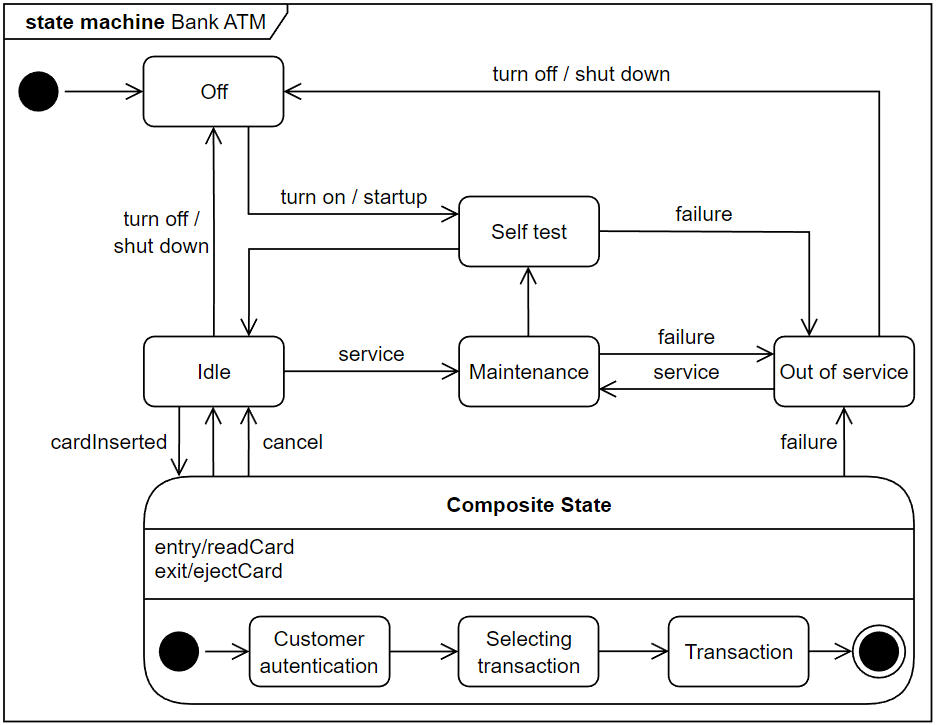
\includegraphics[width=0.75\linewidth]{images/state.png}
    \caption{Example of a state diagram}
\end{figure}
For effective dynamic modeling, it is crucial to construct models solely for classes exhibiting substantial dynamic behavior, considering only relevant attributes. 
Additionally, when deciding on actions and activities, one must account for the granularity of the application and strive to reduce notational complexity.